\documentclass[12pt]{article}

%Packages
\usepackage{titling}
\usepackage{graphicx}
\usepackage{hyperref}
\usepackage{listings}
\lstset{
  language=C, % Set the language to C
  basicstyle=\ttfamily, % Set the font style
  keywordstyle=\color{blue}, 
  commentstyle=\color{green!50!black}, 
  %numbers=left, 
  %numberstyle=\tiny\color{gray},
  %stepnumber=1,
  %numbersep=5pt, 
  breaklines=true, % Allow lines to break
  tabsize=4, % Set tab size
  showspaces=false, % Don't show spaces
  showstringspaces=false % Don't show spaces within strings
}
\usepackage{tikz}
\usetikzlibrary{positioning}

\author{Alessandro Della Siega \\ University of Trieste}
\date{May 2024}
\title{The Mandelbrot set \\ Hybrid MPI/OpenMP implementation}

\pretitle{
    \begin{center}
    \includegraphics[width=0.5\textwidth]{..}\par\vspace{1cm}
    \Huge
}
\posttitle{
    \end{center}
}

\begin{document}

\maketitle

%insert an image in the first page
\begin{figure}[h!]
\centering

\includegraphics[width=0.6\textwidth]{../images/mandelbrot.png}
\caption{Rendering of the Mandelbrot set}
\end{figure}


\section{Introduction}

The OpenMPI library implements several algorithms to perform collective blocking operations according to many different parameters.
OSU Micro-Benchmark is a tool that allows us to evaluate the performance of these operations.

\subsection{Computational architecture}

In order to test the performance of the broadcast and reduce operations, we will use a high-performance computing cluster. The computational resources used to complete the assignment are the ones provided by the ORFEO cluster.

The ORFEO system architecture consists of different machines architecture, in this project the THIN partition is used. The THIN partition consist of 12 Intel nodes: two equipped with Xeon Gold 6154 and 10 equipped with Xeon Gold 6126 cpus.

\subsection{OSU Micro-Benchmark}

OMB includes benchmarks for various MPI blocking
collective operations (Allgather, Alltoall,Allreduce, Barrier, Bcast, Gather, Reduce, Reduce-Scatter, Scatter and vector collectives). These benchmarks work in the following manner. Suppose users run the osu Bcast benchmark with N processes, the benchmark measures the min, max and the average latency of the MPI\_Bcast collective operation across N processes, for various message lengths, over a large number of iterations. In our experiments, we will consider the average latency for each message length.

In this report, two operations are take into consideration: broadcast and reduce.


\subsection{Broadcast}

The broadcast operation \texttt{MPI\_Bcast} is a one-to-all communication operation which allows a process (typically the root process) to distribute information across many processes. This operation is implemented in OpenMP using different algorithms. The algorithms that are considered in this analysis are:
\begin{itemize}
    \item \textbf{basic linear}, the root process sends to all the other process the message without segmentation;
    \begin{center}
    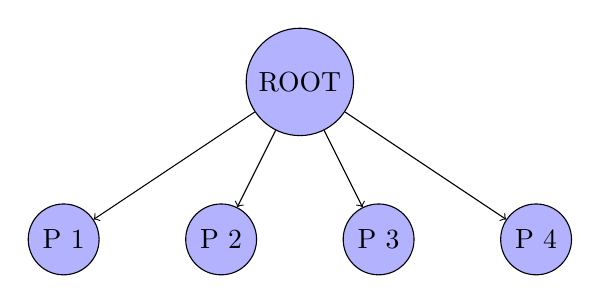
\begin{tikzpicture}
        [
        level distance=2cm,
        sibling distance=2cm,
        every node/.style={circle, draw, fill=blue!30},
        edge from parent/.style={->,draw}
        ]
        % Root node
        \node {ROOT}
        % Level 1: Children nodes
        child { node {P 1} }
        child { node {P 2} }
        child { node {P 3} }
        child { node {P 4} };
    \end{tikzpicture}
    \end{center}

    \item \textbf{chain}, the message is split into segments and transmission of segments continues in a pipeline until the last node gets the broadcast message. ith process receives the message from the $(i-1)$-th process, and sends it to $(i+1)$-th process;
    
    \begin{center}
    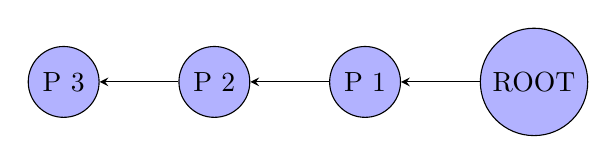
\begin{tikzpicture}[
        every node/.style={circle, draw, fill=blue!30},
        <-, >=stealth
        ]
        % Define the nodes
        \node (n1) {P 3};
        \node (n2) [right=of n1] {P 2};
        \node (n3) [right=of n2] {P 1};
        \node (n4) [right=of n3] {ROOT};
      
        % Draw the arrows
        \draw (n1) -- (n2);
        \draw (n2) -- (n3);
        \draw (n3) -- (n4);
    \end{tikzpicture}
    \end{center}

    \item \textbf{split binary tree}, suppose that each process is a node of a binary tree and the root node is the root process, each parent node sends the message to its children. As the name of the algorithm suggests, the message is split in two halves before transmission and when each half of the message reaches its destination, it is necessary to merge the two halves.
    \begin{center}
        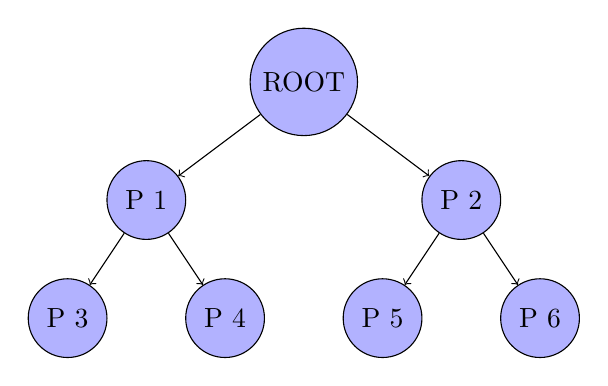
\begin{tikzpicture}[
            level 1/.style={sibling distance=4cm},
            level 2/.style={sibling distance=2cm},
            every node/.style={circle, draw, fill=blue!30, minimum size=1cm},
            edge from parent/.style={->, draw}
            ]
            % Root node
            \node {ROOT}
              % Level 1
              child { node {P 1}
                % Level 2
                child { node {P 3} }
                child { node {P 4} }
              }
              child { node {P 2}
                % Level 2
                child { node {P 5} }
                child { node {P 6} }
              };
          \end{tikzpicture}
    \end{center}

\end{itemize}


\subsection{Reduce}

The reduce operation \texttt{MPI\_Reduce} combines the elements provided in the input buffer of each process in the grouping the specified operation, and returns the combined value in the output buffer of the root process. The specific operation used to reduce the input in the OSU benchmark are sum, maximum, and minimum.

The algorithms that are considered in this analysis are:
\begin{itemize}
    \item \textbf{basic linear}, the root process receives the message from all the other process and reduces the messages;
    \item \textbf{chain}, if we order the processes with respect to their rank, each process sends the message to the next process, each process receives the message from the previous process and reduces the messages;
    \item \textbf{binary tree}, suppose that each process is a node of a binary tree and the root node is the root process. Each parent node receives the message from its children and reduces the received messages passing the result to its parent node.
\end{itemize}
\section{Implementation}

\subsection{Encoding}
The encoding of the problem is straightforward. An image of the Mandelbrot set is a two-dimensional array of pixels. Each pixel corresponds to a point in the complex plane. However, the image is stored as a one-dimensional array of pixels. Each pixel is stored as a \texttt{unsigned char}, its maximum value can be 255. This means that the maximum iteration that can be reached on a point of the Mandelbrot is 255. A scale of gray is used to represent the points of the Mandelbrot set. For each pixel we will assign a value based onn wether the corresponding point belongs to the mandelbrot set: 
\begin{itemize}
    \item if the point belongs to the Mandelbrot set, the pixel is assigned the value 0 and the pixel will be black;
    \item if the point does not belong to the Mandelbrot set, the pixel is assigned the iteration count at which the point exited the circle of radius 2. The pixel will be assigned a value between 1 and 255 and the pixel will be colored according to the gray scale.
\end{itemize}

\subsection{C implementation}
Let us present a brief summary of C implementation:
\begin{itemize}
    \item \texttt{main.c}, it contains the main function in which MPI is initialized, the amount of work is distributed among the MPI processes, and the computation is performed. In the end, the computation is gathered and the image is saved. The main function also takes care of the timing of the computation;
    \item \texttt{mandelbrot.c}, in this file we define two functions. The first is the iterative quadratic map that characterizes the points of the Mandelbrot set. The latter is  the function whose task is to evaluate, within an OpenMP parallel region, the Mandelbrot set on a given array of pixels;
    \item \texttt{image\_utils.c}, in this file we define the function that saves the image in the desired PGM format;
    \item \texttt{timing\_utils.c}, here the function that saves the timing results on a \texttt{.csv} file.
\end{itemize}


\subsection{MPI parallelization}

In order to distribute the work among the MPI processes we decided to adopt a sequential fashion.

Suppose to have $P$ processes and $N = n_x \times n_y$ pixels to compute. The root process divides the one-dimensional array in $M$ blocks of approximately $N/M$ pixels each. Obviously, the last block may contain less pixels if $M$ is not divisible by $N$ since the remainder is distributed starting from the first process, with respect to the rank. The first process is assigned the first block of pixels, the second process the second block, and so on. The last process is assigned the last block of pixels. The gathering of the results is done by the root process, which calls \texttt{MPI\_Gatherv} to collect the results from all the other processes and saves the image.

\subsection{OpenMP parallelization}

The OpenMP parallelization is performed in \texttt{compute\_mandelbrot\_set} in the file \texttt{mandelbrot.c}. The parallel region is defined at the beginning of the function and the parallel for directive is used to parallelize the loop that iterates over the pixels of the image, i.e. the elements of the one-dimensional array. The scheduling policy is set to \texttt{dynamic}: OpenMP assigns one iteration to each thread. When the thread finishes, it will be assigned the next iteration that has not been executed yet.

\subsection{Experimental setup}

For what concerns the timing of the computation, we will use the \texttt{MPI\_Wtime} function to measure the time spent in the computation of the Mandelbrot set. In particular, For each run, we start the timer after the MPI initialization and stop it right after the gathering of the results. In our measures we do not include the time required to save the image on a file since we are not interested in the I/O performance.

Now, for what concerns the scaling analysis, we will consider the following setup. For both the MPI and OpenMP scaling, we will consider the strong scaling and the weak scaling. The strong scaling consists in fixing the dimension $n_x, n_y$ of the Mandelbrot image and increasing the number $P/T$ of processes/threads. While, the weak scaling consists in fixing the amount of work per process/thread and increasing the number of processes/threads.
Let us define the following setup:
\begin{itemize}
    \item \textbf{MPI strong scaling}: we fix $T=1$,
        $$n_x = 4096$$
        $$n_y = 4096$$
    and $P = 1, 2, 4, 8, 16, 32, 64, 80, 96, 112, 128$.
    \item \textbf{MPI weak scaling}: we fix $T=1$, 
        $$n_x = 1024 \times \texttt{round} \{\sqrt{P}\}$$
        $$n_y = 1024 \times \texttt{round}\{\sqrt{P}\}$$
    for $P = 1, 2, 4, 8, 16, 32, 64, 80, 96, 112, 128$;
    \item \textbf{OpenMP strong scaling}: we fix $P=1$,
        $$n_x = 4096$$
        $$n_y = 4096$$
    for $T = 2, 4, 6, 8, ... 62, 64$;
    \item \textbf{OpenMP weak scaling}: we fix $P=1$
        $$n_x = 1024 \times \texttt{round}\{\sqrt{T}\}$$
        $$n_y = 1024 \times \texttt{round}\{\sqrt{T}\}$$
    for $T = 2, 4, 6, 8, ... 62, 64$.
\end{itemize}.

For the MPI scaling, we set \texttt{--map-by core} since we want that, after that a node is selected, each process spawns in its cores.

For the OpenMP scaling, we used the default option \texttt{--map-by socket} since we are using a single process and a single socket which has 64 cores. Lastly, we set \texttt{OMP\_PLACES=cores} to minimize resource contention: assigning threads to distinct cores helps to minimize contention for CPU resources, ensuring that each thread has dedicated compute power
\section{Results}

In this section we will discuss the results obtained from the scaling analysis.

\subsection{MPI scaling}

The results obtained The MPI strong scaling seems to scale well up to 128 processes as shown in Figure \ref{fig:mpi_strong_scaling}. This is confirmed by the speedup which is perfectly linear. The discrepancy between the ideal and the actual strong scaling is low. The nature of the Mandelbrot set computation allow us to compare our results to the ideal scaling. By ideal scaling we mean the Ahmdal's law in which we assume that the entire work is parallelizable and there is no communication overhead. 

The MPI weak scaling, after 10 processes reaches a plateau. This means that the speedup is constant as the number of processes increases as shown in Figure \ref{fig:mpi_weak_scaling_speedup}. This is reasonable since the amount of work per process is constant and also the time is constant as the number of processes increases.

\begin{figure}[h!]
    \centering
    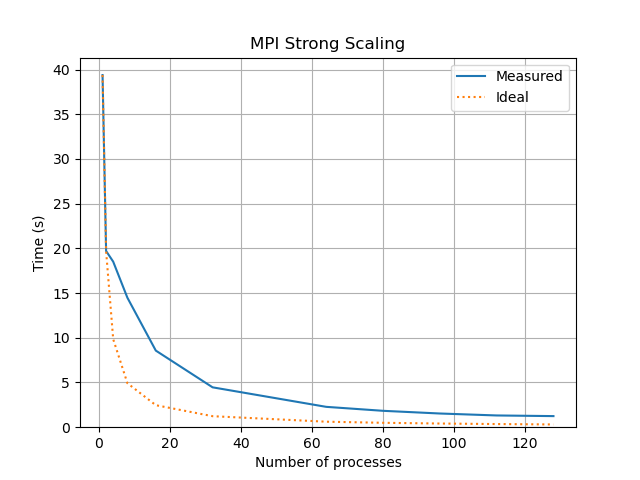
\includegraphics[width=0.8\textwidth]{../images/mpi_strong_scaling.png}
    \caption{MPI strong scaling}
    \label{fig:mpi_strong_scaling}
\end{figure}

\begin{figure}[h!]
    \centering
    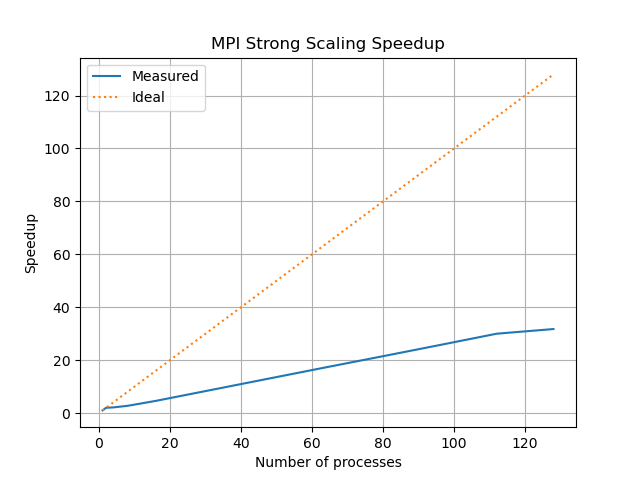
\includegraphics[width=0.8\textwidth]{../images/mpi_strong_scaling_speedup.png}
    \caption{MPI strong scaling speedup}
    \label{fig:mpi_strong_scaling_speedup}
\end{figure}


\begin{figure}[!h]
    \centering
    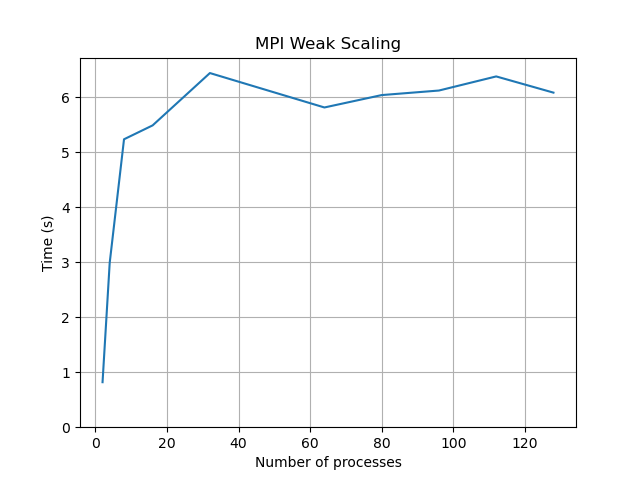
\includegraphics[width=0.8\textwidth]{../images/mpi_weak_scaling.png}
    \caption{MPI weak scaling}
    \label{fig:mpi_weak_scaling}
\end{figure}

\begin{figure}[h!]
    \centering
    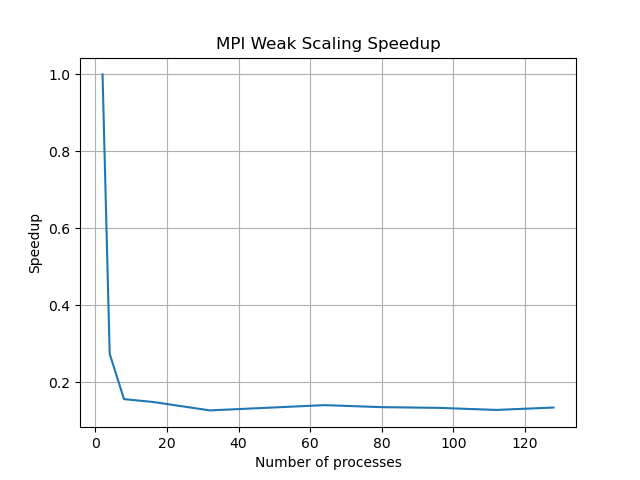
\includegraphics[width=0.8\textwidth]{../images/mpi_weak_scaling_speedup.png}
    \caption{MPI weak scaling speedup}
    \label{fig:mpi_weak_scaling_speedup}
\end{figure}


\subsection{OpenMP scaling}

The OpenMP strong scaling seems to scale with some more overhead than the MPI strong scaling. However, there is a substantial discrepancy between the ideal and the actual strong scaling as shown in Figure \ref{fig:openmp_strong_scaling}. After 20 threads the speedup decreases and becomes constant. This means that the overhead is significantly larger than the computation time.

For what concerns the OpenMP weak scaling, the speedup becomes constant as the number of threads increases as shown in Figure \ref{fig:openmp_weak_scaling_speedup}. We can notice that in this case the scaling assumes a step-like shape. This is due to the fact that we decided to round the square root of the number of threads to the nearest integer to make the amount of work per thread approximately equal.

\begin{figure}[h!]
    \centering
    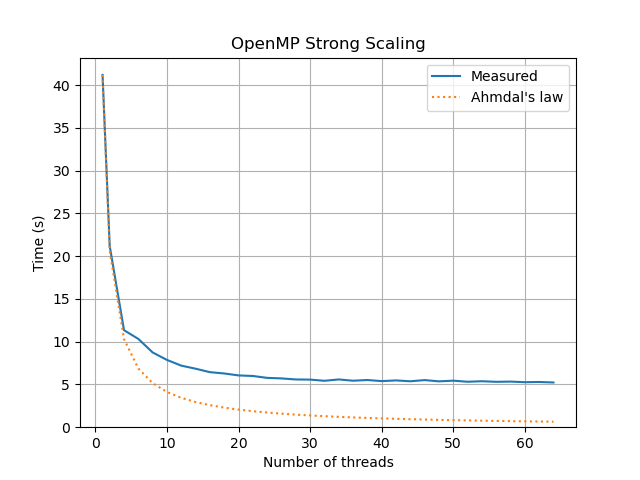
\includegraphics[width=0.8\textwidth]{../images/omp_strong_scaling.png}
    \caption{OpenMP strong scaling}
    \label{fig:openmp_strong_scaling}
\end{figure}

\begin{figure}[h!]
    \centering
    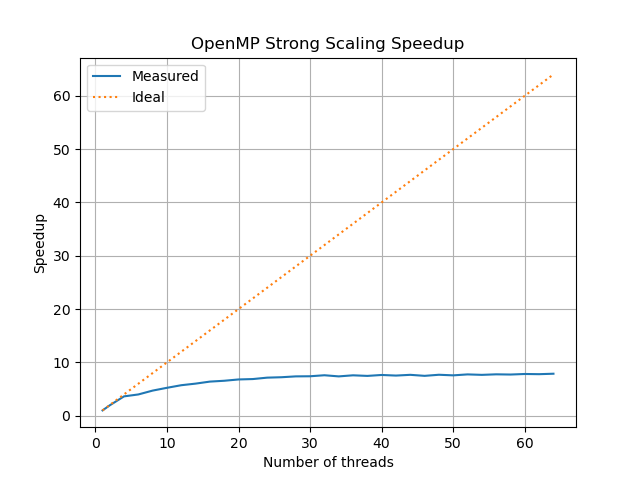
\includegraphics[width=0.8\textwidth]{../images/omp_strong_scaling_speedup.png}
    \caption{OpenMP strong scaling speedup}
    \label{fig:openmp_strong_scaling_speedup}
\end{figure}

\begin{figure}[h!]
    \centering
    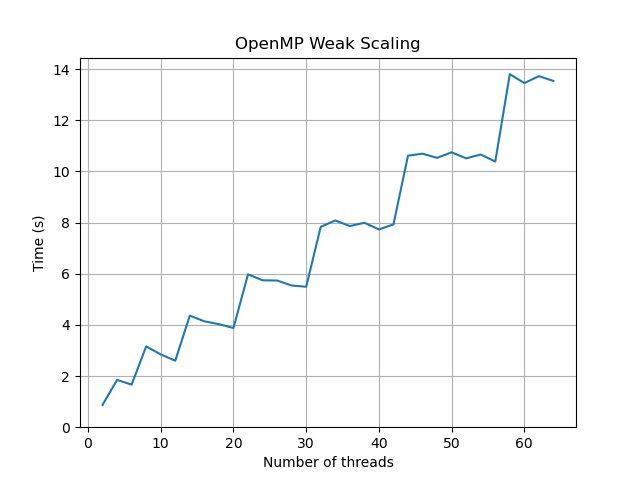
\includegraphics[width=0.8\textwidth]{../images/omp_weak_scaling.png}
    \caption{OpenMP weak scaling}
    \label{fig:openmp_weak_scaling}
\end{figure}

\begin{figure}[h!]
    \centering
    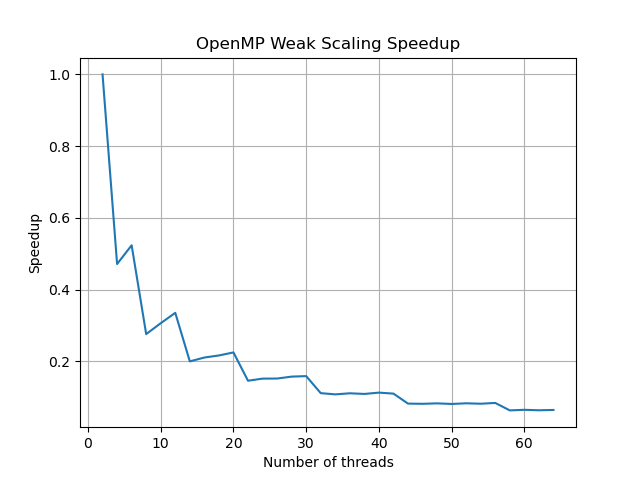
\includegraphics[width=0.8\textwidth]{../images/omp_weak_scaling_speedup.png}
    \caption{OpenMP weak scaling speedup}
    \label{fig:openmp_weak_scaling_speedup}
\end{figure}




\section{Conclusion}

Within this assignment we explored a parallel approach for computing the Mandelbrot set, developing an hybrid MPI+OpenMP code. The designed solution seems to scale as expected and the results are consistent with the theoretical expectations.

However, there are some important considerations to be made:
\begin{itemize}
    \item The OpenMP strong scaling shows a substantial discrepancy between the ideal and the actual strong scaling. This can be explained by the following reasons:
    \begin{enumerate}
        \item the workload is unbalanced among the threads. Some regions of the Mandelbrot set require more iterations to be computed than others. This is due to the fact that the Mandelbrot set is a fractal and the convergence rate is different for each point;
        \item the overhead of the OpenMP parallelization is larger than the computation time. This is due to the fact that the OpenMP parallelization is not efficient for small workloads. The overhead of the parallelization is larger than the computation time. Probably, this implementation of considered not large enough images to be computed in parallel.
    \end{enumerate}
    \item The MPI scaling seems to scale as expected. In particular, the use of collective operations, such as \texttt{MPI\_Gatherv}, allows to gather the results in a more efficient way than using point-to-point communication.
\end{itemize}

Some possible improvements to the code could be:
\begin{itemize}
    \item Subdividing the image in a more balanced way among the threads. This could be done by using a more sophisticated partitioning algorithm. For example, we could use a space-filling curve to divide the image in a more balanced way. However, this could make the implementation very complex;
    \item Exploiting some symmetry properties of the Mandelbrot set. The Mandelbrot set is symmetric with respect to the real axis. This means that we could compute only the upper half of the image and then mirror the results to obtain the lower half. This could reduce the amount of work to be done;
\end{itemize}
    


\end{document}